\documentclass[a4paper,DIV=12,BCOR=7mm,abstract=yes,twoside,10pt]{scrreprt}

\author{Joshua Clark}

\usepackage{amsmath}
\usepackage{amssymb}
\usepackage[citestyle=authoryear]{biblatex}
\usepackage{backnaur}
\usepackage{url}
\usepackage{algorithm2e}
\bibliography{references}
\usepackage{booktabs}
\usepackage{tikz}
\usepackage{multicol}

\usepackage{graphicx}
\usepackage[unicode=true,bookmarks=true,bookmarksnumbered=false,bookmarksopen=false,breaklinks=true,pdfborder={0 0 0},colorlinks=false]{hyperref}
\hypersetup{pdftitle={E-Mail Header Information}, pdfauthor={Joshua Clark}}

\usepackage{fancyvrb}
\usepackage{listings}
\usepackage{xcolor}
\usepackage{epigraph}
\usepackage{framed}
\usepackage{lmodern}
\usepackage[T1]{fontenc}
\usepackage{chngcntr}

\lstset{basicstyle=\ttfamily, escapeinside=||, columns=flexible}

\usepackage{listings}
\lstnewenvironment{example}[1][]{
    \renewcommand*{\lstlistingname}{E-Mail Header Fragment}
    \lstset{fancyvrb=true,basicstyle=\ttfamily,captionpos=b,#1}
}{}


\allowdisplaybreaks{}

\counterwithout{figure}{chapter}
\counterwithout{table}{chapter}

\pagenumbering{roman}
\begin{document}

\thispagestyle{empty}

\begin{center} \begin{minipage}[c]{0.75\linewidth} \centering %University
\includegraphics[width=0.4\linewidth]{oxford}

\vspace{2cm} %Thesis title
{\uppercase{\Large{}Understanding Information\\Leakage in E-Mail Headers}{\Large \par}} \vspace{2cm}
%Author's name
{\Large{}Joshua Clark}{\Large \par}

\vspace{2cm} %Degree
{\Large{}Fourth Year Project Report for the Final Honour School of
Computer Science}{\Large \par}

\vspace{2cm} %Date
{\Large{}May 2016} %
\end{minipage} \par\end{center}

\cleardoublepage 
\chapter*{Abstract}

After extensive public education, fewer people are now clicking on links in
e-mails that are disguised as phishing attacks, though the threat still
remains, and considerable amounts of work has gone into exploring the
demographics most likely to be targeted.  As the number of technically
literate people grows, this sort of attack is increasingly unlikely to be
successful.  Therefore, malicious entities are more likely to attempt to
attack people based on the information leaked in their emails, and more
specifically, the header, which most people are less likely to have some
degree of control over.

The risks are not just limited to individual users, and at a corporate
level, the risks posed by leaking information through e-mails could be even
greater: e-mail headers can reveal the internal network structure of a
company's computer systems as well as the different pieces of software that
are running inside the system.  Extracting the social information could be
of great value for executing a phishing attack, however, there is also value
in determining the specific weaknesses in a system.  This can be aided
through the use of vulnerability databases.

This report discusses the existing research into the information leaked by
e-mail headers and presents a tool to extract such information.
\cleardoublepage 
\chapter*{Acknowledgements}

I want to thank my supervisor, Dr Jason R.C. Nurse for his assistance
throughout the year; my tutor, Professor Peter Jeavons, for his unfailing
help and support throughout my time at Oxford.  I would like to thank the
residents and chaplains of the Oxford University Catholic Chaplaincy.
Finally, I would like to acknowledge the support from my family and
partner, Agata Borkowska, for encouraging me.

\cleardoublepage 
\tableofcontents 
\let\LaTeXStandardClearpage\clearpage
\let\clearpage\relax  % Do nothing when a \clearpage command appears 

\listoftables \listoffigures \listofalgorithms

\let\clearpage\LaTeXStandardClearpage % Return to the old definition


\chapter{Introduction}\label{chap:int}
\pagenumbering{arabic}
\setcounter{page}{1}

\section{Motivation}

E-mail systems are now so integrated into our modern lives that we struggle to
cope without them.  E-mails ubiquity is also one of its largest weaknesses, a
fact recognised very early on.  The first spam email was sent in 1978, as
documented by~\cite{templeton}.  After spam came phishing, first described
by~\cite{felix1987system}, with the first-real world use being against the
customers of America Online, an ISP.\@  However, this still relies on the
targets providing their data for malicious purposes. One of the first e-mail
viruses to spread was the Happy99 virus, which, other than propagating itself,
had no other effect on infected systems. Later viruses would target credit-card
and banking information. However, all of these techniques rely on the malicious
email being received and its contents being opened.  There are fewer instances
recorded, however, of the information flow being sent the other way.  A more
subtle attack will focus on the information being sent from a legitimate user to
an attacker. It is easy enough for an individual to read an e-mail header and
identify interesting elements, however, on a large scale, this quickly becomes
more difficult.

\section{Aims and Objectives}

This project aims to  support a better understanding of the data that may leaked
when e-mails are sent, both from a personal perspective, as well as the corporate
data that is leaked concern network configurations and software installations.

To support this, I will develop a tool that can be used as described above to
automatically extract information from e-mail headers and analyse its results to
display the personal information contained within an e-mail's header, as well as
information about the software configurations that may be found on a user's
computer, or the servers used to send their e-mail.

The tool's objectives will be to parse, analyse and visualise the contents of
any e-mail header that it is given.  The parsing process should correctly and
efficiently convert the plaintext of an e-mail header into an abstract
representation.  In the analysis section, the representation of the header
should be searched to find information out about the sender, their software and
device, and information for any servers that the e-mail message passes through.
Finally, the visualisation produced should clearly show the information that is
available about the sender of an e-mail and the path the e-mail took in order to
arrive at its final destination.

\section{Structure}

Chapter~\ref{chap:exres} begins by discussing the existing research on
the subject as well as existing publicly-available tools to analyse
headers.  I then use these as a basis to discuss features that would be
expected to appear in a header analyser looking for leaked information
and vulnerabilities.

The specification and design of a program to support the understanding of the
information leaked in e-mail headers is discussed in Chapter~\ref{chap:des}.
The implementation's high-level structure and details will be discussed in
Chapter~\ref{chap:imp}, and algorithms presented in pseudo-code where
necessary.  A full listing will be presented at the end of this document in
an appendix. The results of the analysis of the headers will be discussed in
Chapter~\ref{chap:test}, beginning with the methodology used, and presenting
a number of results, finishing with conclusions and areas of further improvement.

\cleardoublepage \chapter{Literature Review}\label{chap:exres}

In this chapter, we will discuss the nature of existing threats to data, and
the ongoing research in this area.  We will then consider the specific threats
posed by e-mail.

\section{General Data Leakage}

The importance of data leakage is gaining more importance as the amount of
information stored about entities increases, and the risks are being considered
more carefully.  From the obvious ramifications for businesses discussed in
\cite{papadimitriou2011data}: the loss of trust and legal action resulting from
the discovery of leaking data, to the more personal issues discussed in
\cite{irani2011modeling}: the possibility of using the discovered data to
discover passwords or to physically identify them.  53\% of Americans can be
uniquely identified by their birth date, gender and location (city/town), with
the number jumping 87\% when using birth date, gender and zip code.

\subsection{Personal Data Leakage}

From a personal perspective, there are a number of risks.  There are a
significant number of social networks available, with an estimated 1.65 billion
monthly active users, with a significantly higher proportion used in developed
countries.  \cite{irani2011modeling} showed the rate at which the information
gathered from social networks can be used to uniquely identify an individual.

\cite{irani2011modeling} defines the aggregate normalised attribute leakage as 
\[\Psi(F_a,P)=\frac{\sum_{f_a\in F_a}\phi\left(f_a, P\right)}{|F_a|}
\text{ where }\phi\left(f_a, P\right) = \left[f_a\in P\right]\]
for a user's social footprint $P$, and attributes are referenced as $f_a$.

Only 9 sites are required before there is approximately a 0.7 attribute
leakage, corresponding to a 70\% probability that both a person's hometown and
name could be recovered.  A similar number of sites can give an aggregate
normalised attribute leakage of 1, where it becomes almost certain that an
individual may be uniquely identified.

\subsection{Corporate Data Leakage}

When companies receive user data, they often have a legal obligation to ensure
that the data is protected and treated as confidential and sensitive.  When
this trust is broken, there are often severe consequences, both from regulators
and consumers moving their business to competitors.

In addition to ensuring that human procedures are present to ensure the
integrity and confidentiality of data, it is also necessary to ensure that
robust technical measures are in place to prevent data breaches. 
\cite{2016_data_breach_category_summary_2016} lists a total of 12 million data
records from 399 breaches as having been illegitimately accessed in 2016 to date.
Two fifths of these data records are connected to government or military data breaches,
with a third linked to medical and healthcare data, and a further fifth connected
to business data.

\cite{squicciarini2010preventing} considers one way that data may be leaked,
despite care being taken to ensure that it is properly encrypted and stored: by
failing to protect against the indices for databases being stored insecurely,
customer data may be leaked.  Order-preserving encryption schemes, as described
in~\cite{agrawal2004order}, is one way of solving this problem, to an extent.

\section{Data Leakage from E-Mails}

\subsection{E-Mail Headers}

All e-mails include additional information about the sender and receiver, some
of which is used by an e-mail client in order to display more information about
the message that is currently being viewed, such as its original sender,
reply-to addresses and the time it was sent.  Additional fields allow senders
to authenticate themselves using public-key methods.

The format of e-mail headers was first defined in RFC~822, and further refined
in subsequent RFCs.  The standard for e-mails was then formalised precisely in
RFC~5322.

\subsection{Example Header and Pertinent Data}

In the example below, and text highlighted with red, \colorbox{red!30}{like so}
is information about the receiver.  Information about the sender, their
hardware or software is highlighted in green, \colorbox{green!30}{like so}; and
information gathered about intervening devices is highlighted in blue,
\colorbox{blue!30}{like so}.

\begin{example}[caption=Sample E-Mail]
Delivered-To: |\colorbox{red!30}{joshuaclark94@gmail.com}|
Received: by |\colorbox{blue!30}{10.25.150.146}| with |\colorbox{blue!30}{SMTP}| id y140csp543137lfd;
	Sat, 6 Feb 2016 08:49:56 -0800 (PST)
X-Received: by |\colorbox{blue!30}{10.112.12.2}| with |\colorbox{blue!30}{SMTP}| id u2mr8302831lbb.145.1454777396580;
	Sat, 06 Feb 2016 08:49:56 -0800 (PST)
Return-Path: <agatabor@poczta.onet.pl>
Received: from |\colorbox{blue!30}{smtpo75.poczta.onet.pl}| (smtpo75.poczta.onet.pl. [|\colorbox{blue!30}{141.105.16.25}|])
	by mx.google.com with |\colorbox{blue!30}{ESMTPS}| id o199si12255636lfb.94.2016.02.06.08.49.56
	for <joshuaclark94@gmail.com>
	(version=TLS1_2 cipher=ECDHE-RSA-AES128-GCM-SHA256 bits=128/128);
	Sat, 06 Feb 2016 08:49:56 -0800 (PST)
Received-SPF: pass (google.com: domain of ********@poczta.onet.pl designates
		141.105.16.25 as permitted sender) client-ip=141.105.16.25;
Authentication-Results: mx.google.com;
spf=pass (google.com: domain of ********@poczta.onet.pl designates 141.105.16.25
		as permitted sender) smtp.mailfrom=agatabor@poczta.onet.pl
Received: from |\colorbox{green!30}{[10.26.196.156]}| (|\colorbox{green!30}{client-8-32.eduroam.oxuni.org.uk}| [|\colorbox{green!30}{192.76.8.32}|])
(Authenticated sender: |\colorbox{green!30}{********@poczta.onet.pl}|)
by |\colorbox{blue!30}{smtp.poczta.onet.pl}| (Onet) with |\colorbox{blue!30}{ESMTPA}| id 3pyKNH4ffyzT6tkv8
for <joshuaclark94@gmail.com>; Sat,  6 Feb 2016 17:49:50 +0100 (CET)
Date: Sat, 06 Feb 2016 16:49:07 +0000
Subject: Test e-mail
Message-ID: <j66i9tkyhy3l4v77erlw1gne.1454777347191@email.android.com>
Importance: normal
From: ***** <********@poczta.onet.pl>
To: Joshua Clark <joshuaclark94@gmail.com>
MIME-Version: 1.0
Content-Type: multipart/alternative;
	boundary="--_com.android.email_1892258509098440"

----_|\colorbox{green!30}{com.android.email}|_1892258509098440
Content-Type: text/plain; charset=utf-8
Content-Transfer-Encoding: base64

CgoKClNlbnQgZnJvbSBteSBTYW1zdW5nIEdhbGF4eSBzbWFydHBob25lLg==

----_|\colorbox{green!30}{com.android.email}|_1892258509098440
Content-Type: text/html; charset=utf-8
Content-Transfer-Encoding: base64

PGh0bWw+PGhlYWQ+PG1ldGEgaHR0cC1lcXVpdj0iQ29udGVudC1UeXBlIiBjb250ZW50PSJ0ZXh0
L2h0bWw7IGNoYXJzZXQ9VVRGLTgiPjwvaGVhZD48Ym9keT48ZGl2IHN0eWxlPSJ3b3JkLWJyZWFr
O2tlZXAtYWxsOyI+PGJyPjxicj48YnI+PGJyPlNlbnQgZnJvbSBteSBTYW1zdW5nIEdhbGF4eSBz
bWFydHBob25lLjxicj48L2Rpdj48L2JvZHk+PC9odG1sPg==

----_com.android.email_1892258509098440--
\end{example}

The particularly interesting portions of the e-mail header include the IP
addresses of the various servers the message has travelled through, allowing
their approximate location to be determined.  Additionally, the information on
the protocol being used and the software being run allows for anyone with access
to mail headers to find more information about the attacks a device and its
software may be vulnerable to.

In Example~\ref{eg:smtp}, indicates that a server with an internal IP address
of \texttt{10.25.150.146} in the Pacific Seaboard Timezone received the e-mail
using the SMTP protocol.

\begin{example}[caption=E-Mail Server configuration information,label=eg:smtp]
Received: by 10.25.150.146 with SMTP id y140csp543137lfd;
	Sat, 6 Feb 2016 08:49:56 -0800 (PST)
\end{example}

In Example~\ref{eg:ip}, a number of pieces of information can be extracted: the
hostname of the sending device is \texttt{client-8-32.eduroam.oxuni.org.uk} with associated
\texttt{192.76.8.32} is on the eduroam network, with a local IP address of
\texttt{10.26.196.156}.

\begin{example}[caption=Information revealed in Received field,label=eg:ip]
Received: from [10.26.196.156] (client-8-32.eduroam.oxuni.org.uk [192.76.8.32])
\end{example}

Further examples from headers that may be particularly interesting include the following examples.

Many Apple iOS devices will include hardware and version names in the \texttt{X-Mailer} field.

\begin{example}[caption=Apple iPhone version,label=eg:app]
X-Mailer: Zimbra 8.6.0_GA_1153 (MobileSync - Apple-iPhone7C2/1305.238)
\end{example}

\subsection{Existing Research}

In~\cite{nurse2015investigating}, the idea of using the information available
in an email header was mooted, turning the previously standard threat of
malware and phishing contained in received e-mails on its head, and instead
presenting the threat in outgoing emails, and the personally identifying
information (PII) contained therein.  Many emails leaked information about
employers, e-mail services and applications used, and IP address.  Initial
examination of a variety of e-mail headers found within my own inbox also
revealed a plethora of information, including phone carriers, preferred
languages, and system usernames.  It is conceivable therefore, that it is
possible to automate at least part of this, and present the information that
can be extracted, in a white-hat tool to allow people to audit the information
that they are revealing.  The obvious malicious use-case involves using such
information as part of a spear-phishing exercise.

An alternative vulnerability presents itself in the information about systems
that may be revealed.  Many email clients embed identifying information, and
there are multiple databases available to allow specific threats to be
identified.  This could allow a malicious entity to compromise the security of
a target machine, and gain access to the data stored on that machine and
available on any connected network devices.  Work started in
\cite{joshi2013extracting} discusses the need to aggregate data about
vulnerabilities from multiple sources to present a more complete and coherent
picture, which is also likely to then contain more accurate data.

\cite{Al-zarouni_tracinge-mail} presents an alternative set of results,
describing how an individual can seek to protect themselves against malicious
e-mails, using the contents of e-mail headers.  Various discrepancies between
forged e-mail addresses and legitimate messages are described.

\section{Existing Tools}

Several tools already exist online to display the information that is found in
e-mail headers.  Tools from Microsoft and Google exist to analyse the contents
of e-mail headers.  These tools clearly display the information displayed in
the header, showing the key-value pairs, and the set of servers the message
transferred through and the protocols used.

\subsection{Google}\label{sec:goo}

The Google Apps Toolbox features an e-mail header analyser\footnote{Found at
	\url{https://toolbox.googleapps.com/apps/messageheader/}}. An example
of the output of the utility is found in Figure~\ref{fig:goo}.

One of the most useful features from the Google Apps Toolbox is the information
provided about the servers the message travelled through.  This tool shows the
details of the time taken for each hop, and the protocol used.

\begin{figure}[ht] \centering
\includegraphics[width=0.9\linewidth]{google-header}
\caption{Google Apps Toolbox E-mail header output} \label{fig:goo}\end{figure}

\subsection{Microsoft}\label{sec:mic}

The Microsoft Message Header Analyser\footnote{Fount at
	\url{https://testconnectivity.microsoft.com/MHA/Pages/mha.aspx}} and
showing sample results in Figure~\ref{fig:mic} is of a similar nature to the
Google tool, discussed in Subsection~\ref{sec:goo}.  In addition to the
information presented by Google, this tool also produces a set of ``Other
Headers'', highlighting fields that may be of interest.  However, little
additional context is provided as to their relevance.

\begin{figure}

	\centering \includegraphics[width=0.9\linewidth]{microsoft-header}

\caption{Microsoft E-mail header output} \label{fig:mic}\end{figure}

\section{Vulnerabilities}

\epigraph{Beware of bugs in the above code; I have only proved it correct, not
	tried it.}{Donald Knuth}

Problems in software are nothing new, and seeking to exploit these issues is
almost as old.   As the security implications behind flawed software became
more widely recognised, reducing their impact wherever possible became the next
most important step.  The MITRE Corporation operates the National Cybersecurity
Federally Funded Research and Development Centre, which exists to maintain a
database of these vulnerabilities, which are referred to as Common
Vulnerabilities and Exposures (CVE).

\subsection{MITRE CVE Lookup}\label{sec:mit}

There are a number of tools to look up CVEs\footnote{Fount at
	\url{https://www.cve.mitre.org/find/index.html}} and showing sample
results in Figure~\ref{fig:cve}.  There are a number of limitations to the
results returned by the CVE Mitre tool.  Firstly, little context is returned:
information about scores, the impact and access information are omitted, for
example.  Additionally, the process of finding relevant vulnerabilities is
further slowed down by the necessity to search for specific terms one at a
time.  Additionally, automated tools exist at a consumer and enterprise level
that will automatically scan a computer or network to detect installed software
configurations and show the results.

\begin{figure} \centering \includegraphics[width=0.9\linewidth]{cve-lookup}
\caption{CVE Search Results}\label{fig:cve} \end{figure}

\subsection{Norton Vulnerability Protection}\label{sec:nor}

For example, the now deprecated Norton Vulnerability Protection tool, as shown
in Figure~\ref{fig:nort}\footnote{Available at \url{community.norton.com}}
lists the programs and the total number of  vulnerabilities found, providing
more information on each program.  This method has the advantage of indicating
the specific programs that have vulnerabilities, with the aim of allowing a
user to update their vulnerable applications, however it does not allow for
more fine-grained information.


\begin{figure}[h!t]  \centering \includegraphics[width=0.9\linewidth]{norton-cve}

	 \caption{Norton Vulnerability Protection Results}\label{fig:nort}
\end{figure}

\section{Summary}

There breadth of research available indicates the importance that is placed on
maintaining data security, as well as the attempts to track and report on
breaches, allowing individuals and companies to track when their data may be
exposed.  There is also a research available on the data that is willingly
disclosed by individuals, and this analyses the risk to individuals that a
malicious actor accumulating this data can present. 

Less research is available on the nature of the data leaked through e-mails,
though it is becoming more common, with information also being provided on ways
to protect against malicious or spoofed e-mails, as well as significant amounts
of work on spam-detection.

There are a number of specific tools available designed to analyse e-mail
headers, however, their main focus is usually on presenting the trace fields,
rather than the information that may be extracted from the rest of the e-mail.

Finally, available tools for analysis of CVEs tend to have divergent aims, with
the tool either being aimed at experienced professionals, offering a lot of
data, but only if the user is familiar with the system of CVEs, or offering
just enough information to allow a system to be kept updated as vulnerabilities
are discovered.
 
\cleardoublepage \chapter{An Approach to Support Understanding of Data Leakage in E-Mail Headers}\label{chap:des}

\section{Overview}

In order to satisfy the aims of this project, and building on the presented
objectives, this chapter discusses the requirements of the software intended to
analyse e-mails and the design of the program and its specifications.

\section{Program Specification}

The software should automatically extract information from e-mail headers and
analyse its results to display the personal information contained within an
e-mail's header, as well as information about the software configurations that
may be found on a user's computer, or the servers used to send their e-mail.

The program would be expected to satisfy the following minimal requirements in
order for it to be considered successful: 

\begin{description} 
	
\item [{Accuracy}] --- any information produced by the parser should be
	reflective of the input e-mail

\item [{Representation}] --- the produced visualisation should be intuitive to
	read: each element should be presented separately from the others, and
	clearly labelled.

\item [{Portability}] --- the visual output produced by the program should be
	available to the user in a variety of formats.

\item [{Interactivity}] --- the program should produce sensible warnings when
	an e-mail that is not possible to parse has been entered.

\end{description}

\section{Program Overview}

The program is split up into three main stages: textual analysis and parsing;
header contents analysis, and visualisation, as shown in Figure~\ref{fig:con}.
The relevant data is often stored in a central \texttt{MainWindow} class,
rather than passed as a parameter, as the composition would indicate, allowing
clear references to be maintained.

The  analysis is implemented as a series of stages, firstly, the e-mail header
is parsed, to extract important information to a predefined set of Java objects.
This is followed by the analysis phase, where the resultant data is passed to a
set of analyser modules, each running separately.  Finally, this information is
presented to the user.  After discussing an overview of each module, this chapter 
presents each of these stages in detail.

\begin{figure}
	\centering
\resizebox{0.9\textwidth}{!}{
\begin{tikzpicture}
	\draw [-{Latex[length=3mm]}] (-3,1.5) -- (0,1.5) node [above, text width=2.5cm, align=center, midway] { Plaintext Header };
	\draw (0,0) rectangle node {Parsing} (4,3);
	\draw [-{Latex[length=3mm]}] (4,1.5) -- (7,1.5) node [above, text width=2.5cm, align=center, midway] { Header Representation };
	\draw (7,0) rectangle node {Analysis} (11,3);
	\draw [-{Latex[length=3mm]}] (11,1.5) -- (14,1.5) node [above, text width=2.5cm, align=center, midway] { Device/User Representation };
	\draw (14,0) rectangle node {Visualisation} (18,3);
	\draw [-{Latex[length=3mm]}] (18,1.5) -- (21,1.5) node [above, text width=2.5cm, align=center, midway] { Visualisation as web page };
\end{tikzpicture}}
\caption{Simplified Control Flow of Application}
\label{fig:con}
\end{figure}

\subsection{Parsing}

This module receives the plain-text of the e-mail as an input, splitting it
into two sections, fields with the ``Received'' tag, and all other fields.
These are then parsed separately.  The other fields are easier to parse, as
they can be loaded into a hash-map, split by the colon.  The trace fields
require a more complex parsing strategy, fully described in
Section~\ref{sec:par}.  This information is then extracted to more abstract
Java objects, allowing the relevant information to be queried on a
device-by-device basis, rather than constantly referring back to the source
text.

\subsection{Analysis}

The analysis of the e-mail headers is handled independently by a number of
small classes, each running asynchronously.  The decision was made to structure
the program in such a way that concurrent operation was possible in order to
prevent blocking operations from limiting the progress of other operations.
This also required care to ensure the separation between the model of the
header and the model of the available information was maintained, as no
guarantees could be placed on which thread was modifying data.

It is in this part of the program that the automated discovery of
vulnerabilities takes place.  An example software configuration string is
\texttt{cpe:/a:cloudbees:jenkins:2.2}, so it is necessary to attempt to convert
found software information.  For example, \texttt{Apple Mail} would become
\texttt{apple:mail} and a search would be performed over the database for
configurations containing that string.


\subsection{Visualisation}

Once the header has been analysed, it is then necessary to present the
information that has been found in a useful and informative manner. Firstly,
the information about the individual sender, such as their name, organisation,
software and usernames, should be presented (where it exists).  The information
about the servers that the e-mail has passed through should then be detailed, 
their address, location and software, as well as relevant vulnerabilities.

Once this has been listed, information about the scores of the vulnerabilities
for each piece of found software, and a listing of the available
vulnerabilities should be made.  By providing a visualisation of the
distribution of the scores assigned to each piece of software conclusions can 
be drawn about the expected severity of future vulnerabilities.

\section{Comparisons to Existing Software}

\paragraph{Google and Microsoft Header Analysers} Both of the tools discussed
in Sections~\ref{sec:goo} and~\ref{sec:mic} produced detailed information on
the servers that are being used to send and received messages, with Google's
tool also clearly reporting when its own servers were used to send a message.
The software should mimic this by providing a similar level of detail on the
devices being used to send information, and extend this by looking up
information on the device's owning organisation.  Additionally, a more
exhaustive search of the other fields should be conducted, so more information
about the sender can be provided than the immediately available details such as
time, sender's e-mail and recipient.

\paragraph{MITRE CVE Lookup and Norton Vulnerability Protection} The tools
discussed in Sections~\ref{sec:mit} and~\ref{sec:nor} are both targeted at very
different demographics.  The MITRE CVE Lookup is designed for IT professionals
and system administrators wishing to gather more information about specific
vulnerabilities and software, requiring knowledge of the software present on a
network or device.  The information presented is also not structured or sorted
in a clear fashion.  Norton's tool, on the other hand, is focused on individual
users who administer their own systems.  The information is presented in such a
way as to warn them as to which software needs updating or patching against a
vulnerability, but provides few details on the nature of the vulnerabilities.

The tool that is described in this report ought to be able to bridge the gap
between these two tools, providing a useful and relevant list of
vulnerabilities, without overloading the information provided, or requiring
complex search terms to be crafted. 

\section{Typical Use}
On starting the application, the user will provide an e-mail that they wish
to have analysed.  This will then be parsed, and some relevant information
presented in a table.

Lastly, an option is available to view the information about security
vulnerabilities in a separate webpage, forming the main output of the
program.

The resultant webpage will be structured as in Table~\ref{tab:format}.  It
will then be possible for the user to click on the representations of the
devices to find out more information.  It will also be possible to search
within the vulnerability list to find more information, as well as filter by
impact and availability details.

\begin{table}[h!t] \centering \begin{tabular}{|cccccc|} \toprule
    \multicolumn{6}{c}{Email Header Information}                                                                                                                                                                                                                                      \\
    \midrule \multicolumn{2}{l}{\begin{tabular}[c]{@{}l@{}}Sender Information\\
    (Name, originating domain)\end{tabular}} & \multicolumn{2}{l}{Sender
    Software} & \multicolumn{2}{l}{\begin{tabular}[c]{@{}l@{}}Sender Usernames\\
    (Presented as a list with likely organisation)\end{tabular}} \\
    \midrule
    \multicolumn{6}{c}{Graphical representation of devices used to deliver the
    e-mail}                                                                                                                                                                                                \\
    \midrule
    \multicolumn{6}{c}{List of derived information including found software and
    similar information}                                                                                                                                                                                  \\
    \midrule
    \multicolumn{6}{c}{Histograms for vulnerability scores, separated by
    product}                                                  \\
    \midrule
    \multicolumn{6}{c}{Table of discovered CVEs that can be searched and filtered}                                                                                                                                                                                                            \\
    \bottomrule \end{tabular} \caption{Format of presented data found in e-mail
    header}\label{tab:format} \end{table}

 
\cleardoublepage \chapter{Implementation}\label{chap:imp}

\section{Overview}

The  analysis is implemented as a series of stages, firstly, the e-mail header
is parsed, to extract important information to a predefined set of Java objects.
This is followed by the analysis phase, where the resultant data is passed to a
set of analyser modules, each running separately.  Finally, this information is
presented to the user.  This chapter presents each of these stages in detail.

\subsection{Program Overview}

The program is split up into three main stages: textual analysis and parsing; header contents analysis, and visualisation, as shown in Figure~\ref{fig:con}.

\begin{figure}[!ht]
	\centering
\resizebox{0.9\textwidth}{!}{
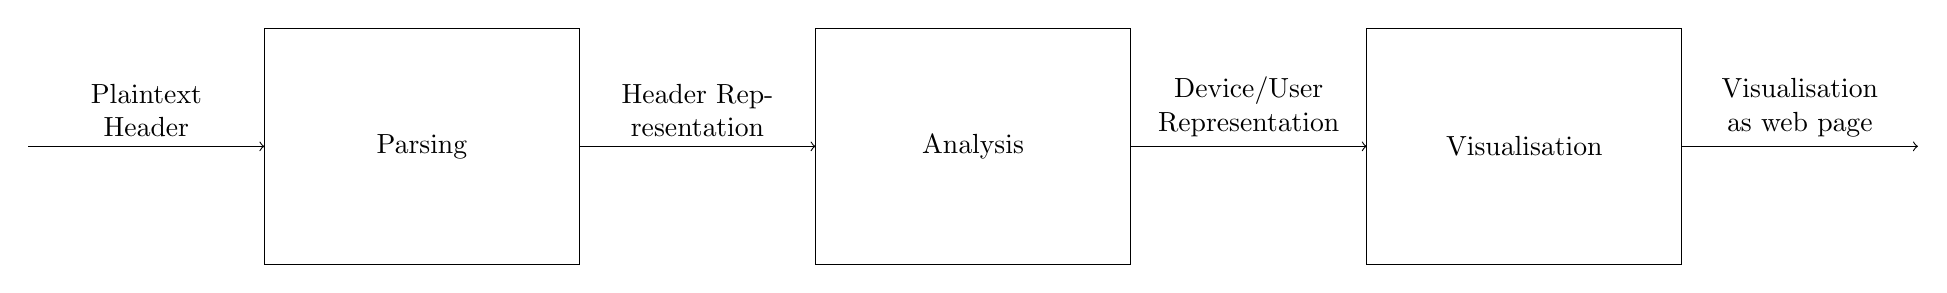
\begin{tikzpicture}
	\draw [->] (-3,1.5) -- (0,1.5) node [above, text width=2.5cm, align=center, midway] { Plaintext Header };
	\draw (0,0) rectangle node {Parsing} (4,3);
	\draw [->] (4,1.5) -- (7,1.5) node [above, text width=2.5cm, align=center, midway] { Header Representation };
	\draw (7,0) rectangle node {Analysis} (11,3);
	\draw [->] (11,1.5) -- (14,1.5) node [above, text width=2.5cm, align=center, midway] { Device/User Representation };
	\draw (14,0) rectangle node {Visualisation} (18,3);
	\draw [->] (18,1.5) -- (21,1.5) node [above, text width=2.5cm, align=center, midway] { Visualisation as web page };
\end{tikzpicture}}
\caption{Simplified Control Flow of Application}
\label{fig:con}
\end{figure}

\section{Definitions}

The following covers the essential definitions required for the notation and
concepts that will be discussed in this document.

\subsection{Parsing}

In order to aid the parsing of the e-mail header, a combination of regular
expressions and context-free grammars are needed, and defined as follows.

\paragraph{Alphabets and Languages}

A set of symbols, usually denoted as $\Sigma$.  A language is a subset of
$\mathcal P (\Sigma)$.

The following special classes are provided as part of the Perl-Compatible
Regular Expression library, and are subsets of the alphabet of Unicode
characters, defined in~\cite{php_group_gutmans_lerdorf_suraski_boerger}.

\begin{description}

\item[alnum] --- letters and digits

\item[alpha] --- letters

\item[ascii] --- the set of ASCII characters (character codes 0 --- 127)

\item[blank] --- tabs or blank spaces

\item[cntrl] --- control characters

\item[digit] --- decimal digits

\item[graph] --- printing characters (excluding spaces)

\item[lower] --- lower-case letters

\item[print] --- printing characters (including spaces)

\item[punct] --- punctuation marks (printing characters excluding letters and spaces)

\item[space] --- white space

\item[upper] --- upper case letters

\item[word] --- ``word'' characters (same

\item[xdigit] --- hexadecimal digits

\end{description}
\subsubsection{Regular Languages}
Regular languages are defined as follows:
\begin{itemize}
\item $\emptyset$ and $\{\epsilon\}$ are regular languages
\item for each $a\in\Sigma$, $\{a\}$ is a regular language
\item if $A$ and $B$ are both regular, $A\cup B$, $A\cdot B$ and $A^*$ are regular languages.
\subitem{ $A\cup B$ is the union of two languages.  $A\cup B = \{s : s\in A \lor s \in B\}$}
\subitem{ $A\cdot B$ is the concatentation of two languages.  $A\cdot B = \{ ab : a \in A, b \in B\}$}
\subitem{ $A^*$ is the Kleene star of a language.}
\begin{align*}
    A_0&=\{\epsilon\}\\
    A_1&= A\\
    A_{i+1} &= \{ aa' : a \in A_i, a'\in A\}\\
    A^* &= \bigcup_{i\in\mathbb N} A_i
\end{align*}
\end{itemize}

\subsubsection{Context-Free Grammars}
A context-free grammar $G$ is defined as $G=\left(V,\Sigma, R,S\right)$ where:
\begin{itemize}
\item $V$ is a variable.
\item $\Sigma$ is the alphabet of symbols.
\item $R$ is a relation defined over $V\rightarrow \left(V\cup\Sigma\right)^*$
\item $S$ is the start symbol
\end{itemize}

For example, $\langle \text S \rangle$ is the field name with the associated
productions $\langle \text T \rangle \, \langle \text U \rangle$, where $T$ and
$U$ are productions.

\begin{bnf*}
	\bnfprod{S}{\bnfpn{T} \bnfsp{} \bnfpn{U}}
\end{bnf*}

For example, $\langle \text S \rangle$ is the field name with the associated
productions $a \, \langle \text U \rangle$, where $a$ is a terminal symbol.

\begin{bnf*}
	\bnfprod{S}{\bnftd{a} \bnfsp{} \bnfpn{U}}
\end{bnf*}
This is then extended in the following ways used in the RFC syntax.

The square brackets are used to indicate an optional element.
\begin{bnf*}
\bnfprod{field}{\bnfpn{field-name} \bnfts{:} \bnfsp{}[ \bnfpn{field-body} ]\bnfsp{} \bnfts{CRLF}}\\
\end{bnf*}

The asterisk is used to indicate an element that appears 0 or more times. $n*$
is used to indicate a component that repeats $n$ or more times.

\begin{bnf*}
\bnfprod{fields}{\bnfpn{dates}\bnfsp \bnfpn{source} \bnfsp 1\!*\bnfpn{destination} \bnfsp * \bnfpn{optional-fields}}\\
\end{bnf*}

The hash-symbol is used to indicate an element that appears a certain number of
times. $m*n$ is used to indicate a component that repeats at least $m$ times and
at most $n$ times.

\begin{bnf*}
\bnfprod{fields}{\bnfpn{dates}\bnfsp \bnfpn{source} \bnfsp 1\!\#\bnfpn{destination} \bnfsp * \bnfpn{optional-fields}}\\
\end{bnf*}

The $|$ is used to indicate a selection between a pair of elements.
\begin{bnf*}
\bnfprod{fields}{\bnfts{a}\bnfor \bnfts{b}}\\
\end{bnf*}

\subsection{Database Queries}
The following notations will be used for the CVE database queries.

\paragraph{Set-Theoretic Operators}
The operators $F\cup G$, $F \cap G$, $F\setminus G$ behave as is expected for
these operators, resulting in the union, intersection and difference of the
sets.  The only proviso being that the atrribute names must match.

\paragraph{Selection} \[\sigma_{\text{product}=\text{thunderbird}}D\]
The above notation is used to indicate a search over the attribute named
``product'' for the string ``thunderbird'' in the database table $D$.  As a
single database is only being used, this may be occasionally elided.  The output
of this function is another object of the same type as $D$.

\paragraph{Projection}
\[\pi_{\text{product}}D\]
The above notation is used to indicate a projection on the attribute named
``product'' in the database table $D$.  The output of this function is another
object of the same type as $D$.

\paragraph{Composition}
The above functions results can be coposed repeatedly to produce more specific
search queries.

\subsection{Data Structures}
These wil be drawn using square boxes to represent single objets that are encapsulated
within an object.  Square boxes with an inner square box indicate some collection
of objects.

Thin arrows will be used to denote the encapsulation relation, with thicker
arrows being used to list relevant public methods.

\section{Data Extraction and Parsing}

The parser's operation completes in a number of stages, following RFC822
(\cite{RFC0822}).  The header is divided up into two disjoint sections, the
routing information (\texttt{Received from...}) and the key-value map of other
pertinent information.

\subsection{Received fields}

The received fields are the most complicated part of the e-mail header to parse,
as they are described by a non-trivial grammar, presented below.

\begin{bnf*}
\bnfprod{message}{\bnfpn{fields}\bnfsp *(\bnfts{CRLF} \bnfsp *\bnftd{text})}\\
\bnfprod{fields}{\bnfpn{dates}\bnfsp \bnfpn{source} \bnfsp 1\!*\bnfpn{destination} \bnfsp * \bnfpn{optional-fields}}\\
\bnfprod{field}{\bnfpn{field-name} \bnfts{:} \bnfsp [ \bnfpn{field-body} ]\bnfsp \bnfts{CRLF}}\\
\bnfprod{field-name}{\bnftd{any word consisting of CHAR, excluding CTLs, SPACE, and ``'':''}} \\
\bnfprod{field-body}{\bnfpn{field-body-contents} \bnfsp [\bnfts{CRLF} \bnfsp \bnftd{LWSP-char}\bnfsp  \bnfpn{field-body}]}\\
\bnfprod{field-body-contents}{\bnftd{ASCII characters}}\\
\bnfprod{source}{[\bnfpn{trace}] \bnfsp \bnfpn{originator} [\bnfpn{resent}]}\\
\bnfprod{trace}{\bnfpn{return}\bnfsp 1\!* \bnfpn{received}}\\
\bnfprod{return}{\bnfts{Return-path:}\bnfsp{} \bnfpn{route-addr}}\\
\bnfprod{recieved}{\bnfts{Received:}}\\
\bnfprod{cont.}{[\bnfts{from}\bnfsp\bnfpn{domain}]}\\
\bnfprod{cont.}{[\bnfts{by}\bnfsp\bnfpn{domain}]}\\
\bnfprod{cont.}{[\bnfts{via}\bnfsp\bnfpn{atom}]}\\
\bnfprod{cont.}{*(\bnfts{with}\bnfsp\bnfpn{atom})}\\
\bnfprod{cont.}{[\bnfts{id}\bnfsp\bnfpn{msg-id}]}\\
\bnfprod{cont.}{[\bnfts{for}\bnfsp\bnfpn{addr-spec}]}\\
\bnfprod{cont.}{\bnfts{;}\bnfsp\bnfpn{date-time}}\\
\bnfprod{msg-id}{\bnfts{$<$}\bnfpn{addr-spec}\bnfts{$>$}}\\
\bnfprod{addr-spec}{\bnfpn{local-part}\bnfsp\bnfts{@}\bnfsp\bnfpn{domain}}\\
\bnfprod{local-part}{\bnfpn{word}\bnfsp *(\bnfts{.}\bnfsp\bnfpn{word})}\\
\bnfprod{word}{\bnfpn{atom}\bnfor\bnfpn{quoted-string}}\\
\bnfprod{domain}{\bnfpn{sub-domain} *(\bnfts{.}\bnfpn{sub-domain})}\\
\bnfprod{sub-domain}{\bnfpn{domain-ref}\bnfor\bnfpn{domain-literal}}\\
\bnfprod{domain-ref}{\bnfpn{atom}}\\
\bnfprod{date-time}{[ \bnftd{day,} ] \bnfsp \bnftd{date}\bnfsp \bnftd{time}}\\
\bnfprod{atom}{1\!*\bnftd{any character excluding specials, SPACE and CTLs}}\\
\end{bnf*}

An example field is as follows:
\begin{verbatim}
Received: from relay12.mail.ox.ac.uk (129.67.1.163)
    by HUB05.ad.oak.ox.ac.uk (163.1.154.231)
    with Microsoft SMTP Server id 14.3.169.1;
    Sat, 14 Nov 2015 10:55:35 +0000
\end{verbatim}
\subsection{Other fields}

These are read by a Python script and output to \texttt{STDOUT} to be read by
the Java parser in a consistent format.  These are then loaded into a hashmap to
allow quick lookup.

\section{Analysis}

After completing the parsing of the fields, it is then ready to be analysed for
different features.  All of the analysers implement the \texttt{HeaderAnalyser}
interface, requiring information about the header to be analysed, and the
currently running application.  All of these then implement the
\texttt{Runnable} interface, allowing the class to be run asynchronously.

\subsection{Input Data Structures}
The data structure presented in Figure~\ref{fig:hea} shows the output of the
parsing and textual analysis module, which is then provided as an input to the
analysis modules.

\begin{figure}[!ht]
\centering
\resizebox{0.9\textwidth}{!}{
	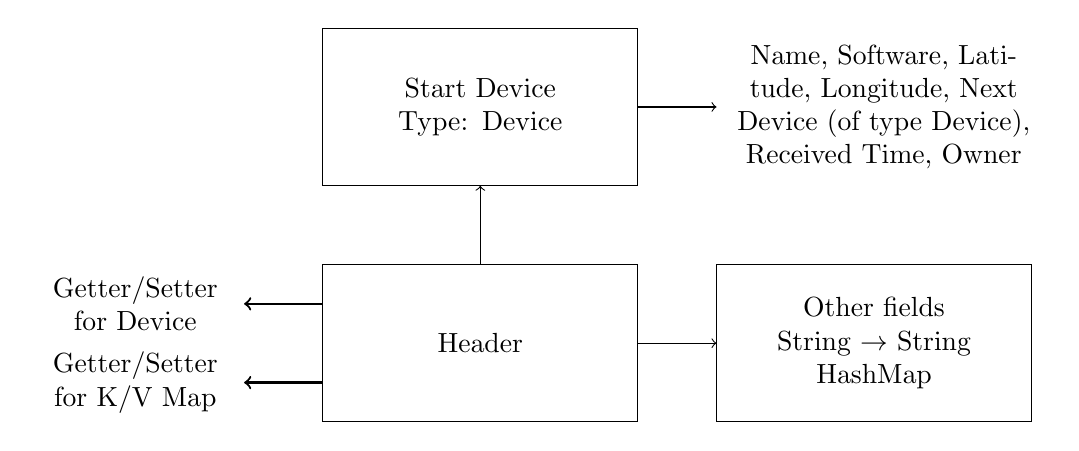
\begin{tikzpicture}
		\draw (0,0) rectangle node {Header} (4,2);
		\draw (0,3) rectangle node [text width = 3.5cm, align=center] {Start Device\\Type: Device} (4,5);
		\draw (5,0) rectangle node [text width = 3.5cm, align=center]
		{Other fields\\String $\rightarrow$ String HashMap} (9,2);
		\draw [->] (2,2) -- (2,3);
		\draw [->] (4,1) -- (5,1);
		\draw [->] (4,4) -- (5,4) node [right, text width = 4cm,align=center] { Name, Software, Latitude, Longitude, Next Device (of type Device), Received Time, Owner};
		\draw [->,thick] (0,1.5) -- (-1,1.5) node [left, text width = 2.5cm,align=center] { Getter/Setter for Device};
		\draw [->,thick] (0,0.5) -- (-1,0.5) node [left, text width = 2.5cm, align=center] { Getter/Setter for K/V Map};
\end{tikzpicture}
	}
	\caption{Header Data Structure Format}
	\label{fig:hea}
\end{figure}

\subsection{Text-Based}

The fields from the header are analysed in different modules, with searches
being performed for specific strings.  Of particular interest to Oxford Nexus
users is the ``X-Oxford-Username'' string, containing the username of the
individual that sent the message.  As confirming the username is a fairly
standard security procedure for an IT support technician, having access to this
information could allow a phisher in a later stage of an attack to increase
their credibility.

In some cases, the likely keys that are being searched for are known in advance,
and can then be checked against the hash-map of entries.

An example of this approach is for the specific check for an Oxford username, as shown in Algorithm~\ref{alg:oxf}.

\begin{algorithm}[!ht]
	\KwIn{Header}
	\KwOut{Any Oxford-based username that is found}
	\If{\texttt{X-Oxford-Username} $\in$ Header.KvMap}{ \Return{Header.KvMap(X-Oxford-Username)}\; }
	\caption{Lookup based on a known key}
	\label{alg:oxf}
\end{algorithm}

Alternatively, we may be interested in properties of the keys, necessitating a search over the keys, as shown in Algorithm~\ref{alg:exc}.

\begin{algorithm}[!ht]
	\KwIn{Header}
	\KwOut{Any information relating to Microsoft Exchange that is found}
	\ForEach{Key $k\in $ Header.KvMap}{
		\If{$k$ starts-with \texttt{X-MS-Exchange}}{
			\Return{Header.KvMap($k$)}\;
		}
	}
	\caption{Lookup based on a key property}
	\label{alg:exc}
\end{algorithm}

\subsection{Client Inferrence}

In \cite{nurse2015investigating}, a number of different e-mail clients were identified based on the header tags that were present. By identifiying these pieces of software likely to be found on a user's machine, we gain a significant amount of information from them, and should therefore devote some effort to correctly identifying them.  Using a number of e-mail samples provided, I have been able to extract examples for a number of different e-mail clients, and use them to infer the client being used.  Using a sample of e-mails, it is possible to find information for additional e-mail clients and senders, such as (but not limited to) PHPMailer and Foxmail.  A number of these approaches are shown in Algorithm~\ref{alg:inf}.

\begin{algorithm}[!ht]
	\KwIn{Header}
	\KwOut{The name of the software that is likely being used, and necessary CVE Product name (elided for brevity)}
	\uIf{``Message-ID''${}\in{}$Header.KvMap}{
		\If{Header.KvMap(``Message-ID'') contains ``email.android.com''}{
			\Return{``Android Device''}\;
		}
	}
	\uElseIf{``X-Mailer''${}\in{}$Header.KvMap}{
		\Switch{Header.KvMap(``X-Mailer'') contains}{
			\Case{``iPhone''}{\Return{``iPhone''}}
			\Case{``Outlook Express''}{\Return{``Microsoft Outlook Express''}}
			\ldots
		}
	}
	\uElseIf{``User-Agent''${}\in{}$Header.KvMap}{
		\Return{``Thunderbird''}\;

	}
	\ElseIf{Header.KvMap${}\cap{}$OutlookKeywords${}\neq\emptyset$}{
		\eIf{``X-Mailer''${}\in{}$Header.KvMap}{ \Return{Apple Mail}}{ \Return{Outlook}}

	}
	\caption{Client Inferrence Technique}
	\label{alg:inf}
\end{algorithm}


\subsection{Database Queries}

Using the results gathered from the text-based queries and analysis of the
received fields, relevant software configurations are extracted and queried
against results in the CVE database.  These are then parsed and collated in
preparation for displaying the outputs. Specifically, the queries are limited
to those matching the product name, and vulnerabilities that can be remotely
executed.

As more information is found, more details of products used will also become
available.  These are added asynchronously.

\begin{algorithm}[!ht]
	\KwIn{Header product name $p$}
	\KwOut{CVE Entries}
	cve-list $\gets\emptyset$\;
	\ForEach{$s\in\sigma_{\text{vector}\neq\text{LOCAL}}\sigma_{\text{product}=p} D$}{
		cve-builder$\gets$blank cve\;
		cve-builder.id$\gets\pi_{\text{CVE-ID}} s$\;
		$\ldots$ -- extract other features\;
		cve-list $\gets$ cve-list${}\cup{}$make(cve-builder)\;
	}
	\Return{cve-list}\;
	\caption{Extracting CVE entries}
\end{algorithm}

\section{Visualising the Results}

Using a pre-existing template, the results from the e-mail analysis will be
presented in a temporary webpage, which can then be saved independently.  Other
than the referenced JavaScript libraries, the document requires no additional
information or database access, allowing it to be quickly shared.

\cleardoublepage \chapter{Evaluation}\label{chap:test}
After producing the application described in Chapter~\ref{chap:imp}, referring
back to the design specifications to determine its performance against the
stated criteria was the next step.  

\section{Methodology}
Using a sample of e-mails provided by my supervisor, each of them was run
through the final version of the program, and scored based on the following
attributes:

\begin{itemize}
\item Let $M$ be the total number of received fields.
\item Let $N$ be the total number of other fields.
\item 1 point is added to the total $R$ for each piece of information found in a Received field for the following:
\subitem{One of device name \emph{or} IP address}
\subitem{Software \emph{or} protocol used}
\subitem{Vulnerabilities found for the relevant piece of software}
\subitem{Location Data}
\item 1 point is addded to $F$ for each piece of information found in other fields.
\end{itemize}

The final score for an e-mail is given as \[\frac12\left(\frac R{4M}+\frac
FN\right)\]to give a value between 0 and 1 for each e-mail.

The e-mails received have been numbered from 1 up to 70, and a random sample of
size 30 was selected using the following code:

\begin{verbatim}
>>> random.seed()
>>> random.sample(list(range(1,70)), 30)
[64, 48, 11, 21, 63, 68, 27, 69, 29,  8, 28,
 34, 13, 57, 10,  3, 22, 32, 23, 49, 26, 45,
 19,  1, 36, 46, 41, 18, 20, 17]
\end{verbatim}

Thus giving a sorted list of the following e-mails: 1, 3, 8, 10, 11, 13, 17,
18, 19, 20, 21, 22, 23, 26, 27, 28, 29, 32, 34, 36, 41, 45, 46, 48, 49, 57, 63,
64, 68, 69.

\section{Results}

Table~\ref{tab:sammn} gives the $M$ and $N$ values for the different sampled
e-mails.  These were sampled using standard Unix tools: \texttt{grep}ping for
fields and counting the output.

\begin{table}
\centering
\begin{tabular}{@{}cccc@{}}
\toprule
Header & Total Fields & $M$ & $N$ \\ \midrule
1.txt  & 26           & 7                     & 19                 \\
3.txt  & 32           & 6                     & 26                 \\
8.txt  & 34           & 8                     & 26                 \\
10.txt & 22           & 3                     & 19                 \\
11.txt & 29           & 6                     & 23                 \\
13.txt & 17           & 4                     & 13                 \\
17.txt & 27           & 6                     & 21                 \\
18.txt & 20           & 6                     & 14                 \\
19.txt & 20           & 6                     & 14                 \\
20.txt & 22           & 7                     & 15                 \\
21.txt & 22           & 6                     & 16                 \\
22.txt & 22           & 6                     & 16                 \\
23.txt & 26           & 6                     & 20                 \\
26.txt & 19           & 6                     & 13                 \\
27.txt & 21           & 1                     & 20                 \\
28.txt & 22           & 6                     & 16                 \\
29.txt & 20           & 6                     & 14                 \\
32.txt & 24           & 6                     & 18                 \\
34.txt & 23           & 5                     & 18                 \\
36.txt & 26           & 6                     & 20                 \\
41.txt & 21           & 6                     & 15                 \\
45.txt & 23           & 6                     & 17                 \\
46.txt & 26           & 5                     & 21                 \\
48.txt & 25           & 6                     & 19                 \\
49.txt & 21           & 6                     & 15                 \\
57.txt & 28           & 6                     & 22                 \\
63.txt & 23           & 5                     & 18                 \\
64.txt & 36           & 9                     & 27                 \\
68.txt & 21           & 6                     & 15                 \\
69.txt & 22           & 6                     & 16                 \\
\bottomrule
\end{tabular}
\caption{$M$ and $N$ values for chosen headers}
\label{tab:sammn}
\end{table}

The results of the testing are contained within Table~\ref{tab:res}, and give a
breakdown for each e-mail's values of $R$ and $F$, as well as the final score.

During the testing, the following trends were noticed.  As many of the e-mails
passed through the same set of servers, as they had been received by an Oxford
e-mail address, the same set of servers were frequently seen, all of which had
associated IP addresses, geolocation data and (except for one server running
Microsoft SMTP Server) CVE data for the running software.  For an e-mail sent
within the University Nexus system, this gives an inflated score, as very few
of the servers are missing information.

The score for the information gathered from fields does not take into account
the number of fields needed to determine or infer a piece of information. For
example, the presence, or absence of multiple fields is required to determine a
piece of information.  Nor does it consider the relative value of a piece of
information, failing to rate the presence of a username above the presence of a
particular piece of software also giving false positives.

However, very few e-mails in the testing population contained fields relating
to usernames (\texttt{X-Oxford-Username}, \texttt{X-}$\ldots$\texttt{-User},
\texttt{X-Authenticated-User}) compared to the result
in~\cite{nurse2015investigating}, which found 14\% of e-mails to contain
usernames as opposed to the 8\% found in the population.

\section{Conclusions}

\section{Future Work}

During the late stages of development and testing, a number of missing features
quickly became apparent. Due to the limited information available, and the
differences in version numbering, a decision was made to search for all
available vulnerabilities for an application, allowing the user to discern
which were most relevant.  Subsequent versions could focus on the different
pieces of version data available.  For example, \texttt{esmtp} frequently
references its version number in the ``Received'' field frequently.

Alternatively, a better picture may be presented by accumulating multiple
e-mails. For example, using the information provided from multiple members of
single organisation, a better picture may be built up of the software used by
the servers, as well as the network configuration.

Additionally, future testing should take place on a larger dataset, using
e-mails from a wider variety of sources sent to a number of different
recipients.  

Finally, it should be possible for an updated version of this application to
determine which header fields have been added by mail servers within one's own
organisation.  For example, e-mail header fields beginning with
\texttt{X-MS-Exchange} are seen within almost all e-mail messages sent to
recipients within the Oxford domain, adding more false positives to the test
results. While it is possible that other preceding e-mail servers have added
similar fields, in most cases, these entries yielded little useful data.

 
\cleardoublepage \printbibliography{} 

\end{document}
